\section{Preliminaries}\label{Section:Preliminaries}
%Preliminaries for the temporal series data analysis: correlograms, partial correlograms. %Preliminaries for the AMIDST models.

\subsection{Dynamic Bayesian Networks}



\begin{figure}
\begin{center}
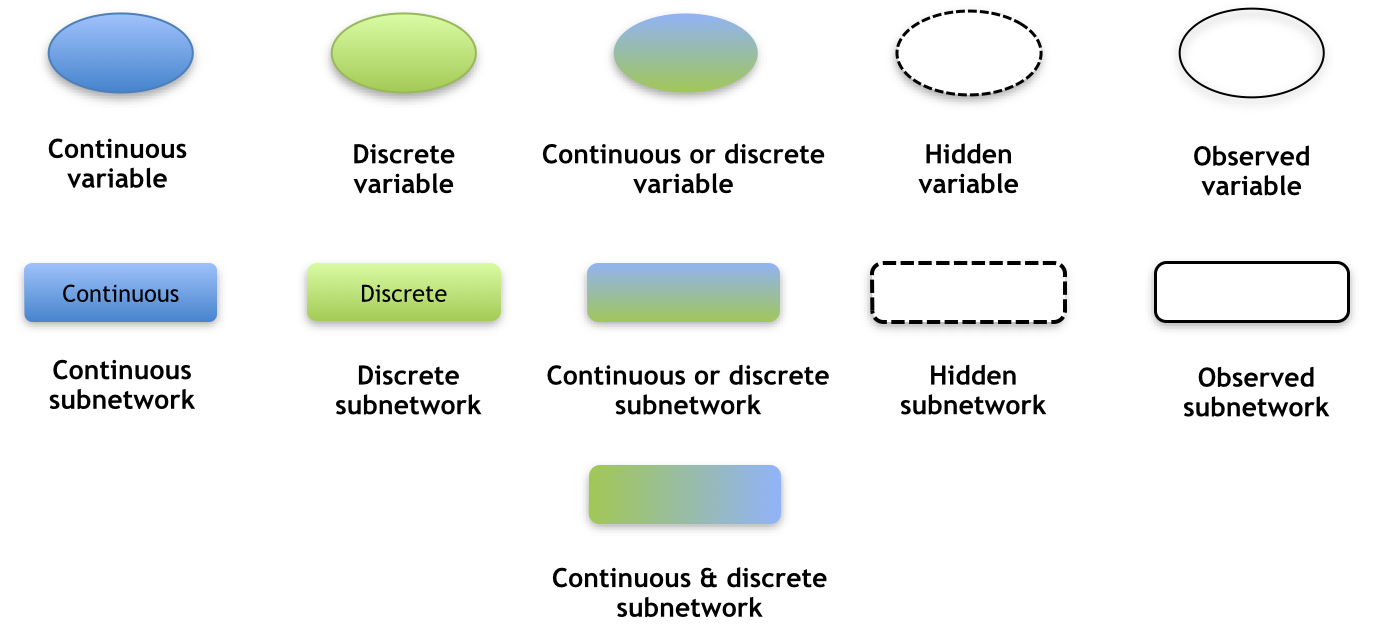
\includegraphics[scale=0.4]{./figures/PreliminariesNotation}
\caption{\label{Figure:PreliminariesNotation}PreliminariesNotation
}
\end{center}
\end{figure}





\subsection{Data Analysis}

As already commented in the introduction, the data analysis detailed here will be used to try to test some of the assumptions supporting the models elicited by the experts in the different use cases, but also to complement our understanding about the nature of the problem we are modelling. The set of tools employed for this purpose try to get insights about some simple and basic aspects of the structural and the distributional assumptions present in a dynamic Bayesian network.


\subsubsection*{Structural assumptions:  Correlograms and Partial Correlograms}

A DBN mainly tries to model complex multivariate time series. By using sample correlogramas and sample partial correlograms we will try to test if the available data support the temporal correlation between variables assumed by the DBN model, i.e. the temporal links between variables. However, these tools will only allow us to look at univariate time series, what strongly limits the reach of the  extracted conclusions. But, at least and as we will see in the different use-cases, this analysis will give us some interesting insights which usually can not be elicited from experts.  


\begin{description}
\item[Sample Correlogram]:  Let ${x_1,...,x_T}$ be a univariate time series. The \emph{sample autocorrelation coefficient at lag v} is given by 

$$ \hat{\rho}_v =\frac{\sum_{t=1}^{T-v} (x_t-\bar{x})(x_{t+v}-\bar{x})}{\sum_{t=1}^{n} (x_t-\bar{x})^2}$$ 

\noindent $\bar{x}$ is the sample mean. The plot of $\hat{p}_v$ versus $v$ for $v=1,...,M$ for some maximum $M$ is called the \textbf{sample correlogram} of the data.

\item[Sample Partial Correlogram]: Let us denote by $X_t$ to the random variable associated to $X$ taking values at time $t$. We can build the following regression problem:

$$ X_t = a_0 + a_1X_{t-1} + a_2X_{t-2} + ... a_{v-1}X_{t-v-1}$$

Let us also denote $e_{i,v}$ to the residuals of this regression problem (i.e. the error when estimating $X_t$ using a linear combination of the $v-1$ previous observations). The \emph{sample partial autocorrelation coefficient of lag v}, denoted by  $\hat{\theta}_v$, is the the standard sample autocorrelation between  the variable $X_{t-v}$ and these residuals. Intuitively, the sample partial autocorrelation coefficient of lag v can be seen as the correlation between $X_t$ and $X_{t+v}$ after having removed the common \textbf{linear} effect of the data in between.
\end{description}


Sample correlograms can be interpreted as a way to measure the strength of the following unconditional dependences: $X_t  \not\perp X_{t+v}$ for some lag $v\geq 1$.  When $\hat{\rho}_v$ is close to zero we have a strong indication that we have an unconditional independence between $X_t$ and $X_{t+v}$. When  $\hat{\rho}_v$ is close to 1 or to -1 we can then say that the correlation or dependency between $X_t$ and $X_{t+v}$ is very strong. But again, we should never forget we are making linear relationships and normality assumptions. 

In Figure \ref{Figure:PreliminariesCorrelograms}, we show an example of how a sample correlogram looks like for two kind of data sets:   a sequence of 50 data samples i.i.d. according to a Gaussian distribution with zero mean and unit variance, $x_t\sim N(0,1)$ (see Figure \ref{Figure:PreliminariesCorrelograms} (a));  and a sequence of 50 data samples distrubted as $x_t=x_{t-1} + \epsilon$, $x_0=\epsilon$, where $\epsilon\sim N(0,1)$ (see  Figure \ref{Figure:PreliminariesCorrelograms} (b)). As can be seen, for the i.i.d. data the correlogram have always values close to zero for all the lags. While for the case of the time series, the correlogram clearly identifies the presence of a temporal relationship in the data. As expected, the correlation decreases with the size of the lag. How quickly it decreases depends of the strength of the temporal relationship. 


Similarly, we plot in Figure \ref{Figure:PreliminariesCorrelograms} (c) and  in  Figure \ref{Figure:PreliminariesCorrelograms} (d) the sample partial correlograms for the same two data sequences. In the case of i.i.d. data, we can see again as the partial correlogram does not show any sign of partial correlation between the samples of the data sequence. However, in the case of the time series data, the partial correlogram take a high value for $v=1$ and then is null for $v$ higher than 1. Sample partial correlogram can be interpreted as a way to measure the strength of the following conditional dependences: $X_t  \not\perp X_{t+v} | X_1,...,X_{t+v-1}$ for some lag $v\geq 1$.  According to that, the sample partial correlogram rightly identify that in this time series data we have the following conditional independencies: $X_t\perp X_{t+2}|X_{t+1}$. So, sample partial correlogram can be seen as a tool to test the order of the Markov chain generating a time data sequence, with all the same caveats expressed for the sample correlogram. 

\begin{figure}
\begin{center}
\begin{tabular}{cc}
(a) Correlogram for i.i.d. data & (b) Correlogram for a time series data \\
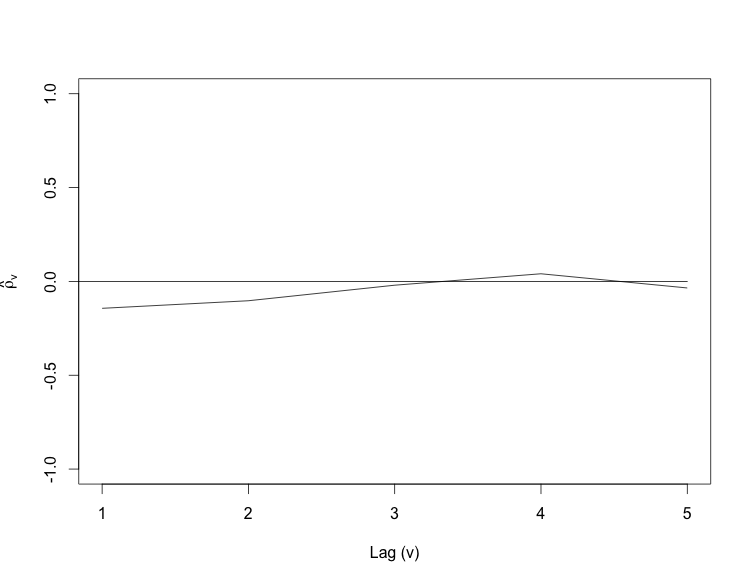
\includegraphics[scale=0.25]{./figures/CorrelogramGaussian} &
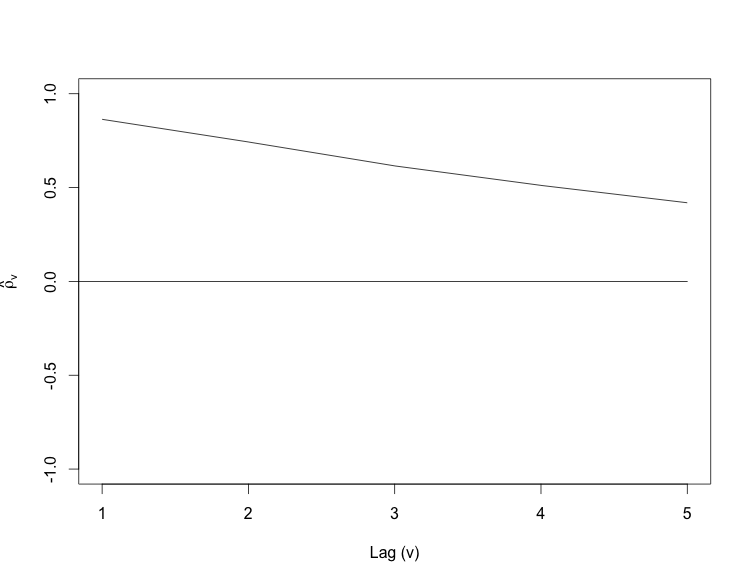
\includegraphics[scale=0.25]{./figures/CorrelogramTimeSerie} \\
(c) Partial Correlogram for i.i.d. data & (d) Partial Correlogram for a time series data \\
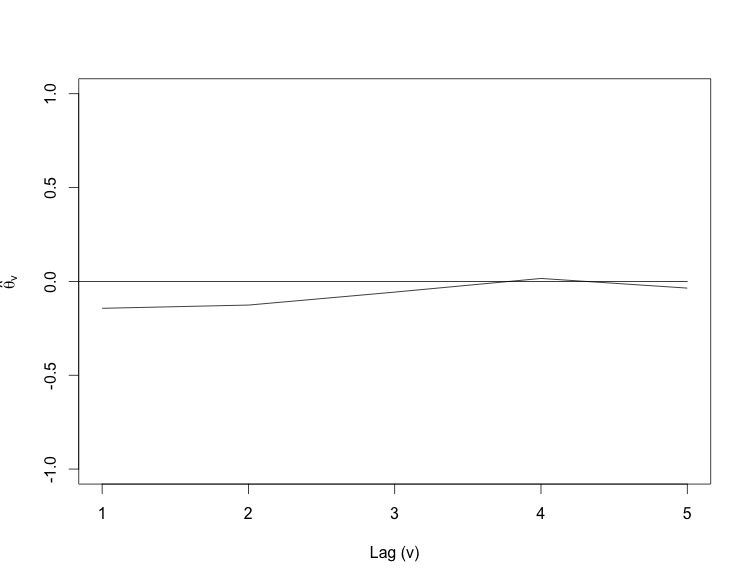
\includegraphics[scale=0.25]{./figures/PartialCorrelogramGaussian} &
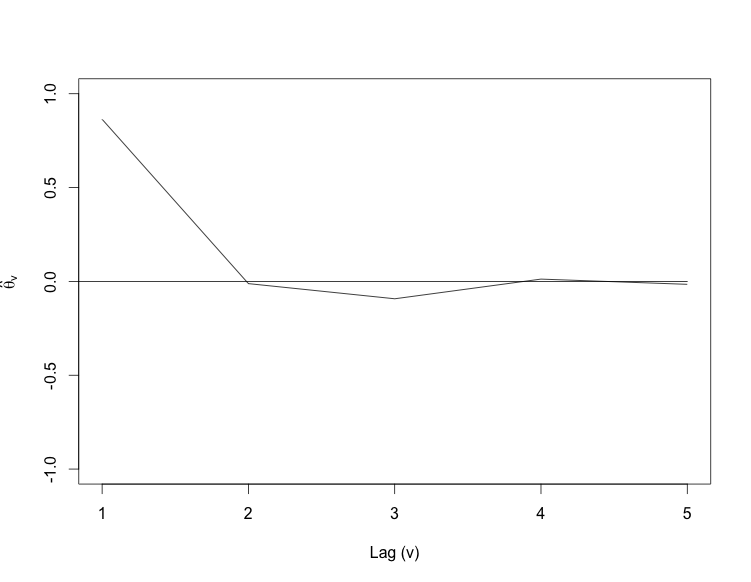
\includegraphics[scale=0.25]{./figures/PartialCorrelogramTimeSerie} \\
\end{tabular}
\caption{\label{Figure:PreliminariesCorrelograms}Sample Correlograms and Partial Correlograms for a set of i.i.d. data and for a time series data. 
}
\end{center}
\end{figure}




\subsubsection*{Distributional assumptions: Histograms and Bivariate Distributions}





For example, we are going to test whether



The aim of the analysis detailed in this section was the following. As commented in the introduction, the models presented from the different use cases were mainly built by expert knowledge. However, when defining these models we did not want to rely only on 
